\chapter{\label{ch:3}Single Cell RNAseq of Human Breast Cancer Cells}

\minitoc

\section{Introduction}

This document introduction won't serve as a complete primer on \LaTeX.  There are plenty of those online, and googling your questions will often get you answers, especially from \url{http://tex.stackexchange.com}.

Instead, let's talk a little about a few of the features and packages lumped into this template situation.  The \verb|savequote| environment at the beginning of chapters can add some wittiness to your thesis.  If you don't like the quotes, just remove that block.

For when it comes time to do corrections, there are two useful commands here.  First, the \verb|mccorrect| command allows you to highlight a short correction \mccorrect{like this one}.  When the thesis is typeset normally, the correction will just appear as part of the text.  However, when you declare \verb|\correctionstrue| in the main \verb|Oxford_Thesis.tex| file, that correction will be highlighted in blue.  That might be useful for submitting a post-viva, corrected copy to your examiners so they can quickly verify you've completed the task.

\begin{mccorrection}
For larger chunks, like this paragraph or indeed entire figures, you can use the \verb|mccorrection| environment.  This environment highlights paragraph-sized and larger blocks with the same blue colour.
\end{mccorrection}

Read through the \verb|Oxford_Thesis.tex| file to see the various options for one- and two-sided printing, including or excluding the separate abstract page, and turning corrections and draft footer on or off, and the separate option to centre your text on the page (for PDF submission) or offset it (for binding).  There is also a separate option for master's degree submissions, which changes identifying information to candidate number and includes a word count.  (Unfortunately, \LaTeX has a hard time doing word counts automatically, so you'll have to enter the count manually if you require this.)

\section{Results}\label{app:imaging}

Within months of Röntgen's discovery of the X-ray in \mccorrect{1895}\cite{gagliardi_rontgen_1996}, cardiac pathology was being investigated via non-invasive imaging \cite{gagliardi_cardiac_1996}.  Over the intervening years, cardiac imaging modalities and techniques have advanced significantly.  Clinically, cardiac imaging is used for two broad purposes: diagnosis of pathophysiology and guidance of interventional procedures.  These applications impose different requirements on imaging equipment, image acquisition time, computational complexity, spatial and temporal resolution, and tissue discrimination.  The common diagnostic and interventional cardiac imaging techniques in current clinical practice are reviewed below.  An accessible introduction to the physics of medical imaging can be found in Webb's \textit{Introduction to Biomedical Imaging} \cite{webb_introduction_2002}.  A comprehensive overview of the use of imaging in clinical cardiology is presented in Leeson's \textit{Cardiovascular Imaging} \cite{leeson_cardiovascular_2011}.

\subsection{Patient Samples and Clinical Characteristics}
I collected three patient samples at the Churchill hospital, Oxford as part of the BRECO study (REC reference 19/SC/0025) between 28th January 2020 - 23rd March 2020. BRECO is a single centre prospective study investigating the relationship between breast cancer and the surrounding tissues. Human tissue, blood samples and clinical data were collected from patients undergoing primary breast surgery. Exclusion criteria included neoadjuvant chemotherapy or radiotherapy.


My sample recruitment focused solely on ER negative, PR negative, HER2 negative invasive breast carcinoma, a rare breast cancer subtype characterised by high levels of intrinsic hypoxia. In order to facilitate sample recruitment for this rare breast cancer subtype, I was actively involved in all stages of patient identification and consent. This patient recruitment process entailed attending the home of a patient on a remote Cotswolds farm (patient consent was obtained for the home visit) or attending pre-operative surgical clinics in Horton General Hospital, Banbury.


The clinical and histological characteristics of the recruited patients are detailed in Table \ref{tab: clinical_characteristics}. Patients were identified for recruitment on the basis of ER/PR/HER2 immunohistochemistry status conducted on the diagnostic breast biopsy performed in the NHS breast cancer triple assessment clinic. All recruited patients were ER 0/8 PR 0/8 HER2 negative in the diagnostic biopsy. However, receptor status can vary when repeated on the definitive final surgical specimen.

\begin{table}[h]
	\centering
	\begin{tabular}{l | l | l}
		Study ID & TNM Stage & Hormone Receptor Status \\
		\hline
		BRECO.BC18 & pT2 50 mm pN1a (1/2) M0 & ER 2/8 PR 0/8 HER2 negative \\
		BRECO.BC20 & pT4 110 mm pN3a (33/33) M1 & ER 0/8 PR 0/8 HER2 negative \\
		BRECO.BC23 & pT3 55 mm pN1a (3/18) M0 & ER 3/8 PR 0/8 HER2 negative
	\end{tabular}
	\caption{Clinical Characteristics}
	\label{tab: clinical_characteristics}
\end{table}

\subsection{Clinical Breast Cancer Samples are amenable for Droplet-based Single Cell RNA Sequencing}
Tumour and non-tumour cells were isolated using the method detailed in chapter 2. The protocol detailed is consistent with the published literature \cite{Bassez2021}.

The key objective for the experimental single cell RNA sequencing pipeline is minimisation of the processing time to enable capture of the native cellular transcriptional state. The objective is a composite function consisting of the synergistic addition of: tissue collection, tissue dissociation to single cell suspension and single cell droplet-based encapsulation. This objective function is given high priority for clinical samples owing to the ethical and practical challenges in sample acquisition.

In the development of the single cell RNA sequencing pipeline for clinical samples, I took active measures to optimise each component. Biopsy specimens were collected intra-operatively. I collected samples directly from within the intra-operative suite and visually inspected each biopsy prior to collection. Repeat biopsies were taken by the surgical team as required.

In order to learn the techniques for single cell RNA sequencing and maximise the potential for successful sample collection, I independently established a new collaboration with Professor Xin Lu at the Ludwig Institute for Cancer Research, Oxford Branch. For all three clinical samples, I worked closely with Dr. Thomas Carroll, a DPhil student in the Lu group who has extensive experience in single cell RNA sequencing conducted as part of a completed trial in oesophageal cancer.

The cellular composition of treatment naive breast cancer, which influences therapeutic response patterns and relapse risk, is an active area of ongoing investigation. I therefore elected against marker-based selection of single cells in order to gain insight into the baseline cellular architecture.

The influence of enzymatic dissociation mixtures on final cell viability and potential bias on gene expression for clinical breast cancer samples is unclear. Therefore, during the processing of sample BRECO.BC18, I compared two enzymatic dissociation mixtures:

i. Mixture A: Collagenase D (Sigma, UK), Liberase DL (Sigma, UK) and DNase I (Sigma, UK). The unpublished protocol was shared by the group of Professor David Tuveson, Cold Spring Harbor Laboratory. This protocol has been successfully used in the dissociation of clinical pancreatic cancer samples and pancreatic cancer organoids.

ii. Mixture B: Miltenyi human tumor dissociation kit (catalogue number: 130-095-929).

Single cell encapsulation, library preparation and downstream analysis was conducted independently to compare the dissociation mixtures. The single cell clusters demonstrated little visual difference between mixture A and B (figure \ref{fig:bro18_dissociation_miltenyi_vs_cshl}). 

Therefore, I adopted dissociation mixture A, a non-propriotary cost-effective option, for all subsequently collected samples.


\begin{figure}
	\centering
	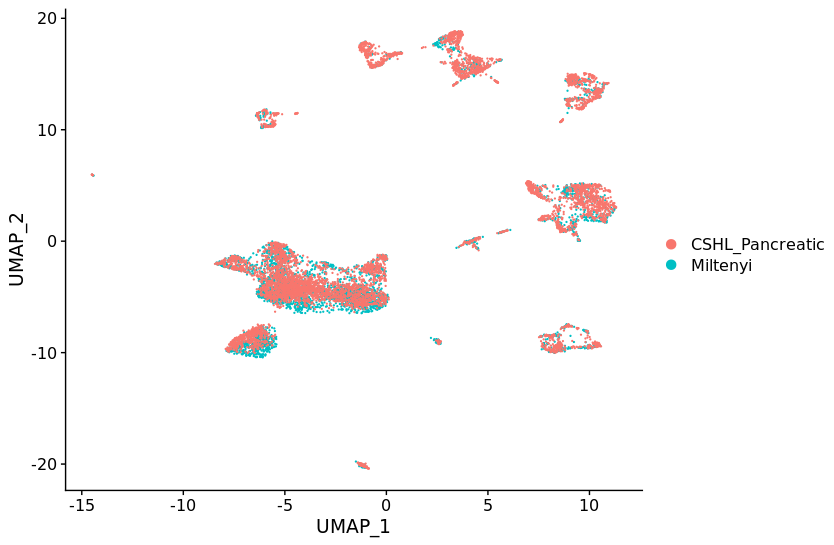
\includegraphics[width=0.7\textwidth]{figures/bro18_dissociation_miltenyi_vs_cshl.png} 
	\caption[Comparison of Dissociation Mixtures.]{UMAP depicting differences between Enzymatic Dissociation Mixtures in Sample BRECO.BC18}
	\label{fig:bro18_dissociation_miltenyi_vs_cshl}
\end{figure}



\subsection{Sample Recruitment in District General Hospitals presents Additional Challenges for the Clinical Single Cell Pipeline}

The BRECO study recruits patients within the Oxford University NHS Foundation Trust catchment area. Therefore, participant treatment can take place in the Churchill hospital, John Radcliffe hospital or Horton General hospital.

The first eligible participant, BRECO.BC15, underwent breast conserving surgery with an intra-operative research biopsy at the Horton General hospital. The geographical spread in the process, participant treatment in Banbury and laboratory facilities in Oxford, presented additional unique challenges since the experimental protocol for single cell RNA sequencing is most effective and efficient when conducted on fresh tissue. I therefore collected the biopsy directly into a vial of warmed Dmem/F12/HEPES medium supplemented with human serum which was immediately placed into a 37 \textdegree{}C water bath within a thermos flask. Mechanical dissociation was facilitated during the journey from Banbury to Oxford by gentle continual rotation of the thermos flask. The entire process required close collaboration with my colleague Miss Ashvina Segaran regarding transfer of equipment and supplies to/from Banbury and with Dr. Thomas Carroll to ensure the prompt continuation of the experimental protocol on arrival back in Oxford. Cell viability was poor at 7\% with the modified protocol and therefore, all subsequent samples were collected exclusively from the Churchill or John Radcliffe hospital.

\subsection{Cell and Gene QC is a Sample Individualised Process}


\subsection{Unsupervised Clustering identifies Cellular Heterogeneity in Human Breast Cancer}
\label{sub:diagnostic}

Beyond the chest X-ray (`plain film'), the key non-invasive imaging modalities in diagnostic cardiology are echocardiography, magnetic resonance imaging, and X-ray computed tomography, which are reviewed below.  Nuclear medicine, including positron emission tomography (PET) and single-photon emission computed tomography (SPECT), are not discussed here, as they do not play a role in the chapters to follow.

\subsection{Characterisation of Human Breast Cancer Cellular Subtypes}







\subsection{Characterisation of Endothelial Heterogeneity in Human Breast Cancer}



\section{Discussion}

\section{Limitations}
